\documentclass{article}
\usepackage{tikz}
\usetikzlibrary{positioning}
\usetikzlibrary{calc}

%%
\usetikzlibrary{shapes.geometric, arrows, positioning}

\tikzstyle{process} = [rectangle, rounded corners, minimum width=2.5cm, minimum height=1cm, draw=black, fill=gray!10]
\tikzstyle{box} = [rectangle, minimum width=2cm, minimum height=1cm, draw=black]
\tikzstyle{arrow} = [thick,->,>=stealth]
\tikzstyle{textlabel} = [align=center]

%%

\begin{document}

\title{TikZ Graph Example}
\author{Your Name}
\date{\today}

\maketitle

\section{Introduction}
This is an example document to create TikZ graphs.

\section{TikZ Graph}


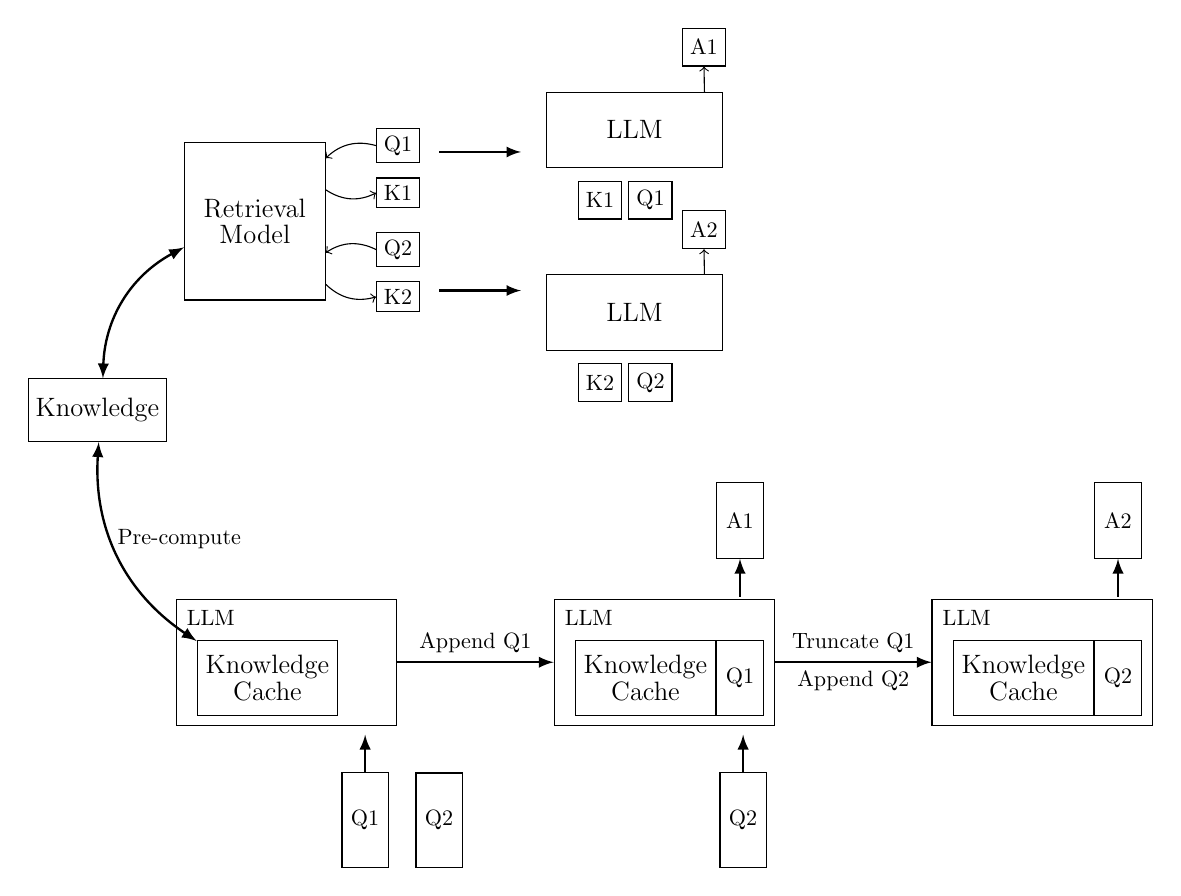
\begin{tikzpicture}[scale=0.8, transform shape]
    % Your TikZ code goes here
    \node[draw, box] at (0, 0) (knowledge) {\large Knowledge};
    \node[
        draw, box, text width=2cm, minimum height=2.5cm, minimum width=2cm, align=center
    ] at (2.5, 3) (retrieval_model) {\large Retrieval Model};
    % \node[draw, box] at (3, 1.5) (retrieval_model) {Retrieval Model};
    
    \draw[<->, latex-latex, line width=0.3mm, bend left] (knowledge) to (retrieval_model);
    
    % \draw[<->] (retrieval_model) to (knowledge_cache);
    
    \coordinate (retrieve_Q1) at ($(retrieval_model.east) + (0cm, 1cm)$);
    \coordinate (retrieve_K1) at ($(retrieval_model.east) + (0cm, 0.5cm)$);
    \coordinate (retrieve_Q2) at ($(retrieval_model.east) + (0cm, -0.5cm)$);
    \coordinate (retrieve_K2) at ($(retrieval_model.east) + (0cm, -1cm)$);
    
    \node (Q1) [draw, rectangle, right=0.8cm of retrieval_model, yshift=1.2cm] {Q1};
    \node (K1) [draw, rectangle, right=0.8cm of retrieval_model, yshift=0.45cm] {K1};
    \node (Q2) [draw, rectangle, right=0.8cm of retrieval_model, yshift=-0.45cm] {Q2};
    \node (K2) [draw, rectangle, right=0.8cm of retrieval_model, yshift=-1.2cm] {K2};
    
    \coordinate (Q1_left) at ($(Q1.west) + (0cm, 0cm)$);
    \coordinate (K1_left) at ($(K1.west) + (0cm, 0cm)$);
    \coordinate (Q2_left) at ($(Q2.west) + (0cm, 0cm)$);
    \coordinate (K2_left) at ($(K2.west) + (0cm, 0cm)$);

    \draw[<-, bend left] (retrieve_Q1) to (Q1_left);
    \draw[->, bend right] (retrieve_K1) to (K1_left);
    \draw[<-, bend left] (retrieve_Q2) to (Q2_left);
    \draw[->, bend right] (retrieve_K2) to (K2_left);

    \node (LLM1) [box, minimum height=1.2cm, minimum width=2.8cm, align=center, right=2cm of Q1, yshift=0.25cm] {\large LLM};
    \node (LLM2) [box, minimum height=1.2cm, minimum width=2.8cm, align=center, right=2cm of K2, yshift=-0.25cm] {\large LLM};
    
    \coordinate (LLM1_Arrow_start) at ($(retrieval_model.east) + (1.8cm, 1.1cm)$);
    \coordinate (LLM1_Arrow_end) at ($(retrieval_model.east) + (3.1cm, 1.1cm)$);
    \draw[-latex, thick] (LLM1_Arrow_start) to (LLM1_Arrow_end);

    \coordinate (LLM1_Arrow_start) at ($(retrieval_model.east) + (1.8cm, -1.1cm)$);
    \coordinate (LLM1_Arrow_end) at ($(retrieval_model.east) + (3.1cm, -1.1cm)$);
    \draw[-latex, thick] (LLM1_Arrow_start) to (LLM1_Arrow_end);


    \node (Q1) [draw, rectangle, minimum height=0.6cm, minimum width=0.4cm, below=0.2cm of LLM1, xshift=0.25cm] {Q1};
    \node (K1) [draw, rectangle, minimum height=0.6cm, minimum width=0.4cm, below=0.2cm of LLM1, xshift=-0.55cm] {K1};
    \node (A1) [draw, rectangle, minimum height=0.6cm, minimum width=0.4cm, above=0.4cm of LLM1, xshift=1.1cm] {A1};
    \coordinate (LLM1_right) at ($(LLM1.east) + (-0.3cm, 0.6cm)$);
    \draw[->] (LLM1_right) to (A1.south);

    \node (Q2) [draw, rectangle, minimum height=0.6cm, minimum width=0.4cm, below=0.2cm of LLM2, xshift=0.25cm] {Q2};
    \node (K2) [draw, rectangle, minimum height=0.6cm, minimum width=0.4cm, below=0.2cm of LLM2, xshift=-0.55cm] {K2};
    \node (A2) [draw, rectangle, minimum height=0.6cm, minimum width=0.4cm, above=0.4cm of LLM2, xshift=1.1cm] {A2};    
    \coordinate (LLM2_right) at ($(LLM2.east) + (-0.3cm, 0.6cm)$);
    \draw[->] (LLM2_right) to (A2.south);


    \node[
        draw, box, text width=2cm, minimum height=2cm, minimum width=3.5cm, align=center
    ] at (3, -4) (LLM1) {};
    \node at ($(LLM1) + (-1.2cm, 0.7cm)$) (LLM1_tx) {LLM};
    \node[
        draw, box, text width=2cm, minimum height=1.2cm, minimum width=2cm, align=center
    ] at ($(LLM1) + (-0.3cm, -0.25cm)$) (knowledge_cache) {\large Knowledge Cache};
    
    \draw[<->, latex-latex, line width=0.3mm, bend right] (knowledge) to (knowledge_cache);
    \node at ($(knowledge_cache) + (-1.4cm, 2.2cm)$) (Precompute) {Pre-compute};
    
    \node[
        draw, box, text width=0.5cm, minimum height=1.5cm, minimum width=0.5cm, align=center
    ] at ($(LLM1.south) + (1.25cm, -1.5cm)$) (LLM1_Q1) {Q1};
    
    \node[
        draw, box, text width=0.5cm, minimum height=1.5cm, minimum width=0.5cm, align=center
    ] at ($(LLM1_Q1.east) + (0.8cm, 0cm)$) (LLM1_Q2) {Q2};
    
    \draw[-latex, line width=0.3mm] (LLM1_Q1.north) to ($(LLM1_Q1.north) + (0cm, 0.6cm)$);
    
    

    \node[
        draw, box, text width=2cm, minimum height=2cm, minimum width=3.5cm, align=center
    ] at (9, -4) (LLM2) {};
    \node at ($(LLM2) + (-1.2cm, 0.7cm)$) (LLM2_tx) {LLM};
    \node[
        draw, box, text width=2cm, minimum height=1.2cm, minimum width=2cm, align=center
    ] at ($(LLM2) + (-0.3cm, -0.25cm)$) (knowledge_cache) {\large Knowledge Cache};
    
    \node[
        draw, box, text width=0.5cm, minimum height=1.5cm, minimum width=0.5cm, align=center
    ] at ($(LLM2.south) + (1.25cm, -1.5cm)$) (LLM2_Q2) {Q2};
    
    \node[
        draw, box, text width=0.5cm, minimum height=1.2cm, minimum width=0.5cm, align=center
    ] at ($(knowledge_cache) + (1.5cm, 0cm)$) (LLM2_Q1) {Q1};
    
    \draw[-latex, line width=0.3mm] (LLM2_Q2.north) to ($(LLM2_Q2.north) + (0cm, 0.6cm)$);
    
    \node at ($(LLM1.east)!0.5!(LLM2.west) + (0cm, 0.3cm)$) (appendQ1) {Append Q1};
    \draw[-latex, line width=0.3mm] (LLM1.east) to (LLM2.west);
    
    
    \node[
        draw, box, text width=0.5cm, minimum height=1.2cm, minimum width=0.5cm, align=center
    ] at ($(knowledge_cache) + (1.5cm, 2.5cm)$) (LLM2_A1) {A1};

    \draw[-latex, line width=0.3mm] ($(LLM2_A1.south) + (0cm, -0.6cm)$) to (LLM2_A1.south);


    \node[
        draw, box, text width=2cm, minimum height=2cm, minimum width=3.5cm, align=center
    ] at (15, -4) (LLM3) {};
    \node at ($(LLM3) + (-1.2cm, 0.7cm)$) (LLM3_tx) {LLM};
    \node[
        draw, box, text width=2cm, minimum height=1.2cm, minimum width=2cm, align=center
    ] at ($(LLM3) + (-0.3cm, -0.25cm)$) (knowledge_cache) {\large Knowledge Cache};
    
    \node[
        draw, box, text width=0.5cm, minimum height=1.2cm, minimum width=0.5cm, align=center
    ] at ($(knowledge_cache) + (1.5cm, 0cm)$) (LLM3_Q1) {Q2};
    
    
    \node at ($(LLM2.east)!0.5!(LLM3.west) + (0cm, 0.3cm)$) (truncateQ1) {Truncate Q1};
    \node at ($(LLM2.east)!0.5!(LLM3.west) + (0cm, -0.3cm)$) (appendQ2) {Append Q2};
    \draw[-latex, line width=0.3mm] (LLM2.east) to (LLM3.west);
    
    
    \node[
        draw, box, text width=0.5cm, minimum height=1.2cm, minimum width=0.5cm, align=center
    ] at ($(knowledge_cache) + (1.5cm, 2.5cm)$) (LLM2_A2) {A2};

    \draw[-latex, line width=0.3mm] ($(LLM2_A2.south) + (0cm, -0.6cm)$) to (LLM2_A2.south);
    
    % \node (CAG_AREA) [draw, rectangle, minimum height=7cm, minimum width=17cm, xshift=0.25cm, dashed]
    %     at (9cm, -4.2cm){};
    
    

\end{tikzpicture}


\end{document}